\documentclass[dvipdfmx,17pt]{beamer}

\usepackage{pxjahyper}
\usepackage{minijs}
\usepackage{amsthm}

\renewcommand{\subset}{\subseteq}
\renewcommand{\emptyset}{\varnothing}

\usefonttheme{professionalfonts}
\mathversion{bold}
\renewcommand{\kanjifamilydefault}{\gtdefault}
%\usetheme{Antibes}
\setbeamertemplate{navigation symbols}{}

\setbeamertemplate{theorems}[numbered]
\setbeamertemplate{footline}[frame number] 


\theoremstyle{plain}
\newtheorem{thm}{定理}
\newtheorem{defi}[thm]{定義}
\newtheorem{lem}[thm]{補題}
\newtheorem{prop}[thm]{命題}
\newtheorem{cor}[thm]{系}
\renewcommand{\proofname}{証明}

\DeclareMathOperator{\Type}{type}

\title{濃度と順序数}


\begin{document}

\begin{frame}\frametitle{}
\titlepage
\end{frame}

\begin{frame}\frametitle{話すこと}
\begin{itemize}
\item 順序数の定義と性質
\item 整列可能定理
\item 濃度の矛盾のない定義
\item Zornの補題の証明
\end{itemize}
\end{frame}

\begin{frame}\frametitle{復習:濃度の定義}
\begin{itemize}
\item 集合$|A|$の濃度とは
\onslide<2->
\item 集合全体の集まりにおける対等関係という同値関係の$A$の同値類のことである
\end{itemize}
\end{frame}

\begin{frame}\frametitle{問題点}
\begin{itemize}
\item 「集合全体の集まり」などと口を濁しているが,要するに「集合全体の集合」を考えている
\item しかし「集合全体の集まり」は集合にはなれない.
\end{itemize}
\end{frame}

\begin{frame}\frametitle{カントールのパラドックス}
\begin{thm}
集合全体の集まりは集合ではない
\end{thm}
\onslide<2->
\begin{proof}
{\small
$V$を集合全体の集合とする.
このときべき集合${\cal P}(V)$は集合の集合なのだから${\cal P}(V) \subset V$.よって$|{\cal P}(V)| \le |V|$	.
一方,カントールの定理より$|V| < |{\cal P}(V)|$.
ここに矛盾した.}
\end{proof}
\end{frame}

\begin{frame}
\begin{itemize}
\item このように「集合全体の集まり」のように大きすぎるものの集まりは集合にならない
\item そこで矛盾のおきない濃度の定義が必要
\item それには順序数という概念を用いる
\end{itemize}
\end{frame}

\begin{frame}
\begin{defi}
順序集合$X$は,すべての空でない部分集合が最小元をもつとき,\textcolor{red}{整列集合}という
\end{defi}
\end{frame}

\begin{frame}
\begin{prop}
整列集合$X$は全順序集合である.
\end{prop}
\onslide<2->
\begin{proof}
任意の2要素$a, b \in X$をとる.
整列集合の定義より,$\{a, b\}$には最小元があるので,$a \le b$または$b \le a$が成り立つ.
よって$X$は全順序集合.
\end{proof}
\end{frame}

\begin{frame}{整列集合の例}
\begin{itemize}
\item $\mathbb{N}$は整列集合
\item 任意の有限の全順序集合は整列集合
\item $\mathbb{Z}, \mathbb{R}$は整列集合でない
\end{itemize}
\end{frame}

\begin{frame}
\begin{itemize}
\item 順序数とは,おおざっぱには「整列集合」の\textcolor{red}{長さ}を測るための数のこと.
\end{itemize}
\end{frame}

\begin{frame}
\begin{itemize}
\item 順序数が定義されたあかつきには,整列集合$X$の型(長さのことを型という)を$\Type X$と書いて,$X \simeq Y \iff \Type X = \Type Y$が成立するようになる.
\end{itemize}
\end{frame}

\begin{frame}
\begin{itemize}
\item 整列集合同士に$X$が$Y$より短いという関係も定義されるのだが,それは$\Type X < \Type Y$と同値になる
\end{itemize}
\end{frame}

\begin{frame}
\begin{itemize}
\item なお,「順序数とは整列集合全体における順序同型という同値関係による同値類のこと」と定義したいが,それもやはり大きすぎる集合を考えることになってダメ.
\end{itemize}
\end{frame}

\begin{frame}
\begin{itemize}
\item 順序数の正確な定義はまだだがイメージを持ってもらおう.
\item 要素数$3$の整列集合というのは以下のハッセ図のものしかない.
\end{itemize}
\begin{center}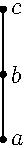
\includegraphics[height=3.5cm]{3.pdf}\end{center}
\begin{itemize}
\item よって要素数$3$の整列集合の型のことを$3$と呼ぶ.

\end{itemize}
\end{frame}

\begin{frame}
\begin{itemize}
\item 同様にして自然数$n$に対して,要素数$n$の整列集合の型のことを$n$と呼ぶ.
\onslide<2-> \item このようにして順序数というのは自然数をすべて含んでいる.
\onslide<3-> \item 順序数というのは自然数が持つ「番号を振る」という目的を無限方向に拡張したものだといえる.
\end{itemize}
\end{frame}

\begin{frame}
\begin{itemize}
\item 整列集合$\mathbb{N}$の型は$\omega$と書かれる.これは最小の無限順序数である.
\onslide<2-> \item 順序数を小さい方から順に並べると$0, 1, 2, 3, \dots, \omega, \omega+1, \omega+2, \omega+3, \dots, \omega2, \omega2 + 1, \dots$となる
\onslide<3-> \item 今並べたのは順序数のうちほんの小さい部分にすぎない.もっと大きい順序数がまだまだある
\end{itemize}
\end{frame}

\begin{frame}
\begin{prop}
整列集合$X$から無限強単調減少列$x_0 > x_1 > x_2 > \dots$はとれない.
\end{prop}
\onslide<2->
\begin{proof}
$x_0 > x_1 > x_2 > \dots$がとれると仮定する.
すると$X$の部分集合$\{x_0, x_1, x_2, \dots\}$には最小元がないため整列性に反する.
\end{proof}
\end{frame}

\begin{frame}
\begin{prop}
順序集合$X \ne \emptyset$が整列集合であるためには,全順序集合であって無限強単調減少列$x_0 > x_1 > x_2 > \dots$がとれないことが必要十分.
\end{prop}
\end{frame}

\begin{frame}
\begin{defi}
整列集合$X$とその要素$a \in X$に対して,
\[X(a) := \{x \in X | x < a \}\]
を$X$の$a$による\textcolor{red}{切片}という.
\end{defi}
\end{frame}

\begin{frame}{切片の例}
\begin{itemize}
\item 整列集合$X = \{0, 1, 2\}$において
\item $X(0) = \emptyset$
\item $X(1) = \{0\}$
\item $X(2) = \{0, 1\}$
\end{itemize}
\end{frame}

\begin{frame}
\begin{lem}
整列集合の部分集合への順序同型$f: (X, \le) \to f(X) \subset X$があれば
\[x \le f(x) \;(\forall x  \in X)\]
\end{lem}
\end{frame}

\begin{frame}
\begin{thm}
\begin{enumerate}
\item 整列集合はどの切片とも順序同型でない
\onslide<2-> \item 整列集合から自身への順序同型は恒等写像に限る
\onslide<3-> \item 整列集合の間の順序同型はあるとしてもひとつしかない
\end{enumerate}
\end{thm}
\end{frame}

\begin{frame}{順序数の定義のアイデア}
\begin{itemize}
\item 順序数とは「それより小さい順序数全体の集合である」ということが成り立つような定義をする
\item このアイデアはJohn von Neumannによるものである.
\end{itemize}
\end{frame}

\begin{frame}
\begin{defi}
整列順序集合$(X, \preceq)$であって
\[X(x) = x \quad(\forall x \in X)\]
をみたすものを\textcolor{red}{順序数}という
\end{defi}
\end{frame}

\begin{frame}{例}
\begin{itemize}
\item たとえば集合$X = \{\emptyset, \{\emptyset\}\}$に$\emptyset \prec \{\emptyset\}$なる順序$\preceq$を入れる
\item $X(\emptyset) = \emptyset$
\item $X(\{\emptyset\}) = \{\emptyset\}$
\item となるので$X$は順序数である.
\end{itemize}
\end{frame}

\begin{frame}
\begin{prop}
順序数$(\kappa, \preceq)$において
\[x \prec y \iff x \subsetneq y\]
が成立する.
\end{prop}
\begin{proof}
{\small
\begin{align*}
x \prec y
&\iff \kappa(x) \subsetneq \kappa(y) \\
&\iff x \subsetneq y
\end{align*}
より成立.
}
\end{proof}
\end{frame}


\addtocounter{thm}{-1}

\begin{frame}
\begin{prop}
順序数$(\kappa, \preceq)$において
\[x \prec y \iff x \subsetneq y\]
が成立する.
\end{prop}
この命題により,順序数$(\kappa, \preceq)$において順序関係$\preceq$はつねに$\subset$と同値になるので,順序関係$\preceq$をあえて指定する必要はない.
よってこれからは順序数$(\kappa, \preceq)$を順序数$\kappa$と書く.
\end{frame}



\begin{frame}
\begin{thm}
順序数$\kappa$の切片はすべて順序数である
\end{thm}

\begin{cor}
順序数$\kappa$の要素はすべて順序数である
\end{cor}
\end{frame}

\begin{frame}
\begin{thm}
相異なる順序数に対して一方は他方の切片である
\end{thm}
\end{frame}

\begin{frame}
\begin{thm}
二つの順序数$\kappa, \tau$が順序同型なら実は$\kappa = \tau$である.
\end{thm}
\end{frame}

\begin{frame}
\begin{thm}
任意の整列集合はただ一つの順序数と順序同型である
\end{thm}
\par \par
整列集合$X$に対してこの順序数のことを$\Type X$と書く.
\end{frame}

\begin{frame}
以上で整列集合と順序数の定義と性質を終える.
\end{frame}

\begin{frame}
\begin{thm}[整列可能定理]
任意の集合$X$は整列可能.
\par \par
すなわち,$X$にある順序関係$\preceq$を入れることで$(X, \preceq)$は整列順序集合になる.

言い換えるとある順序数と$X$には全単射が作れる.
\end{thm}
\end{frame}

\begin{frame}{整列可能定理の証明}
\begin{itemize}
\item $X$に属さない元$\theta$を一つとる.
\item 選択公理により,写像$f: {\cal P}(X) \to X \cup \{\theta\}$で
\[f(\emptyset) = \theta\]
\[\emptyset \ne A \subset X \Rightarrow f(A) \in A\]
となるものをとれる.
\end{itemize}
\end{frame}

\begin{frame}{整列可能定理の証明}
\begin{itemize}
\item $x_0 = f(A)$
\item $x_1 = f(A - \{x_0\})$
\item $x_2 = f(A - \{x_0, x_1\})$
\item $\vdots$
\item $x_\alpha = f(A - \{x_\beta : \beta < \alpha\})$
\item $\vdots$
\item と帰納的に定める.
\end{itemize}
\end{frame}

\begin{frame}{整列可能定理の証明}
\begin{itemize}
\item このとき$x_\tau = \theta$となる$\tau$が存在する.
\item すると$X = \{x_\alpha : \alpha < \tau\}$となり,$X$は整列された. □
\end{itemize}
\end{frame}

\begin{frame}{濃度の定義}

\end{frame}

\begin{frame}
\begin{thm}[Zornの補題]
$X$を空でない部分集合とする.$X$の任意の鎖は上界をもつとする.このとき$X$には極大元が存在する.
\end{thm}
\end{frame}

\begin{frame}{Zornの補題の直観的証明}
\begin{itemize}
\item $x_0 \in X$を一つとる.$x_0$が極大元なら証明終了.
\item そうでないなら$x_1 > x_0$をとれる.$x_1$が極大元なら証明終了.
\item そうでないなら$x_2 > x_1$をとれる.$x_2$が極大元なら証明終了.
\end{itemize}
\end{frame}

\begin{frame}{Zornの補題の直観的証明}
\begin{itemize}
\item 同様に続けて$x_0, x_1, \dots, x_n, \dots$が得られて,まだ極大元がないとする.
\item すると$\{x_0, x_1, \dots, x_n, \dots\}$は$X$の鎖なのでその上界$x_\omega$がとれる.
\item $x_\omega$が極大元なら証明終了.そうでなければ$x_{\omega + 1} > x_\omega$がとれる.
\item 同様のことを繰り返せばいつか極大元が見つかるであろう. □
\end{itemize}
\end{frame}

\begin{frame}
ちゃんとした証明もつけます
\end{frame}

\begin{frame}{Zornの補題の証明}
\begin{itemize}
\item $X$から$X$への写像$^+$で次を満たすものを考える.
\begin{align*}
x^+ > x &\; (\text{もし$x$が極大元でないとき}) \\
x^+ = x &\; (\text{もし$x$が極大元のとき})
\end{align*}
\item 選択公理よりこのような写像$^+$を一つとれる.
\end{itemize}
\end{frame}

\begin{frame}{Zornの補題の証明}
\begin{itemize}
\item $X$の元の広義単調増加列$(x_\alpha)$ ($\alpha$: 順序数)を次のように帰納的に定める.
\item $x_0 = (\text{$X$の元の一つ})$
\item $x_{\beta+1} = {x_\beta}^+$
\item $x_{\alpha} = (\text{鎖($x_\beta)_{\beta < \alpha}$の上界の一つ})$ ($\alpha$が極限順序数のとき)
\end{itemize}
\end{frame}

\begin{frame}{Zornの補題の証明}
\begin{itemize}
\item $X$に極大元がないと仮定する
\item すると列$(x_\alpha)$は狭義単調増加列になる
\item このとき順序数全体が$X$のある部分集合と1対1に対応する
\item しかし,順序数全体は集合にならないのでこれは矛盾 □
\end{itemize}
\end{frame}


\begin{frame}{参考文献}
\begin{itemize}
\item 寺澤順 『現代集合論の探検』
\item “alg\_dによる「選択公理⇒Zornの補題」の概略”

\url{http://togetter.com/li/967760}
\item Ken Brown “Zorn's Lemma”

\url{http://www.math.cornell.edu/~kbrown/6310/zorn.pdf}
\end{itemize}
\end{frame}



\end{document}